\section{Lecture 4: Decision Making I}

The previous lectures described how the brain builds useful representations, selects information, resolves ambiguous percepts, and combines uncertain cues. Decision making adds the next step: the system must convert uncertain evidence into an action. The central problem is not only that the world state is hidden. It is that actions have consequences, evidence is noisy, and sometimes the system can buy more evidence only by spending time or effort.

The mental model for this lecture is a belief state connected to a policy. A sensory measurement \(x\) changes belief about a hidden state \(s\). A reward function \(R(s,a)\) says what each action \(a\) is worth if the state is \(s\). A policy \(\pi(a\mid x)\) maps the current evidence, or the posterior belief inferred from it, to an action. The main question is which policy should be used when the evidence is uncertain.

The Summer Lecture 4 deck develops this question in five linked steps:
\begin{itemize}
    \item Bayesian decision making, where actions are chosen by expected reward;
    \item continuous motor decisions, where an intended movement creates a lottery over possible outcomes;
    \item signal detection theory, where sensitivity is separated from decision criterion;
    \item sequential evidence accumulation, where a log-likelihood ratio is updated sample by sample;
    \item drift-diffusion and reaction-time models, where the retained decision variable explains both accuracy and response time.
\end{itemize}

\subsection{Bayesian decisions as expected-reward policies}

The problem solved by Bayesian decision theory is that the most likely state and the best action need not be the same thing. A medical test may make infection more likely than no infection, but the decision to quarantine also depends on the costs of false alarms, missed infections, and waiting for another test. The same structure applies to perceptual decisions and movements: evidence updates belief, but rewards determine what to do with that belief.

Let
\[
  s \in \{A,B\}
\]
denote the hidden state of the world. In the lecture's diagnostic-test example, \(A\) can mean infection and \(B\) no infection. Let \(x\) denote the evidence, such as a test result or a sensory measurement. The prior
\[
  p(s)
\]
is the probability of each state before the current evidence is observed. The likelihood
\[
  p(x\mid s)
\]
is the distribution of evidence values expected under each state. Bayes' rule gives the posterior belief
\[
  p(s\mid x)
  =
  \frac{p(x\mid s)p(s)}{p(x)},
  \qquad
  p(x)=\sum_{s'}p(x\mid s')p(s').
\]
The denominator \(p(x)\) is the evidence probability. Its role is normalization: after seeing \(x\), the posterior probabilities over the states must add to one.

Now add actions. Let \(a\in\{Y,N\}\), where \(Y\) and \(N\) are the two available reports or interventions. The reward
\[
  R(s,a)
\]
is the payoff obtained if action \(a\) is taken and the true state is \(s\). The expected reward of action \(a\) after observing \(x\) is
\[
  \langle R\rangle(a\mid x)
  =
  \sum_s p(s\mid x)R(s,a).
\]
This equation is the core object in the first part of the lecture. Each posterior probability says how much weight to give a possible state, and each reward says how good the action would be in that state. The optimal deterministic policy chooses the action with the larger expected reward:
\[
  a^*(x)
  =
  \operatorname*{arg\,max}_{a\in\{Y,N\}}
  \langle R\rangle(a\mid x).
\]

\begin{figure}[!htbp]
\centering
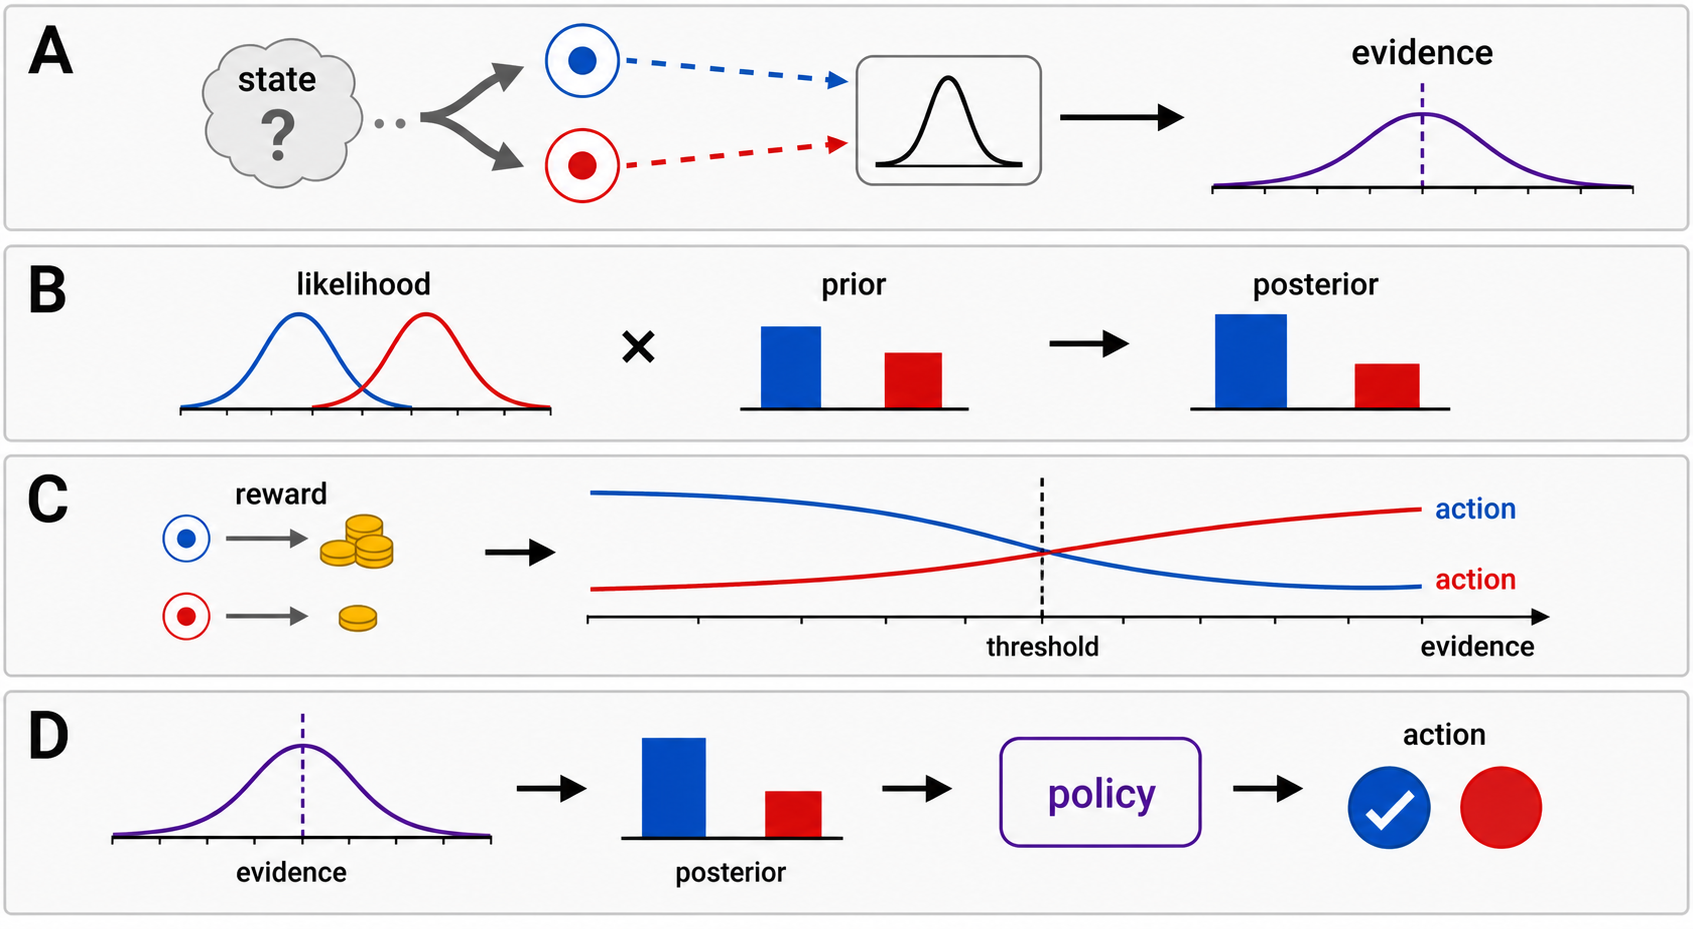
\includegraphics[width=0.96\textwidth]{figures/mhbf-lecture4-bayesian-policy.png}
\caption{Bayesian expected-reward policy. The hidden state generates noisy evidence, the likelihood and prior determine the posterior, rewards convert posterior belief into expected value for each action, and the policy chooses the action whose expected reward is largest.}
\end{figure}

For two actions, it is useful to write the difference in expected reward:
\[
  \Delta R(x)
  =
  \langle R\rangle(Y\mid x)-\langle R\rangle(N\mid x)
  =
  \sum_s p(s\mid x)\bigl(R(s,Y)-R(s,N)\bigr).
\]
If \(\Delta R(x)>0\), choose \(Y\). If \(\Delta R(x)<0\), choose \(N\). The optimal decision criterion is the evidence value \(c\) where \(\Delta R(c)=0\). At this value the two actions have equal expected reward.

Substituting Bayes' rule makes the roles of likelihood, prior, and reward explicit:
\[
  \Delta R(x)
  =
  \frac{1}{p(x)}
  \sum_s p(x\mid s)p(s)\bigl(R(s,Y)-R(s,N)\bigr).
\]
The factor \(1/p(x)\) is positive, so it does not affect which action wins. The sign of \(\Delta R(x)\) is controlled by the prior-weighted and reward-weighted likelihoods.

\paragraph{Practical implication.}
A response bias is not automatically a mistake. If one state is more common, or if one error is more costly, an optimal observer should shift the decision threshold. A clean analysis therefore estimates both the quality of evidence and the policy that turns evidence into action.

\subsection{Decision criteria from priors and payoffs}

The problem now is to turn the reward rule into a criterion that can be fit from data. The analytical exercise gives the boundary for a two-state, two-action task:
\[
  p(x\mid s=A)p(s=A)(R_{AY}-R_{AN})
  =
  p(x\mid s=B)p(s=B)(R_{BN}-R_{BY}).
\]
The left side is the weighted advantage of answering \(Y\) when state \(A\) is true. The right side is the weighted advantage of answering \(N\) when state \(B\) is true. The boundary is where these two advantages exactly balance.

Assume the exercise's equal-variance Gaussian likelihoods,
\[
  p(x\mid s=A)
  =
  \frac{1}{\sqrt{2\pi}}
  \exp\!\left[-\frac{(x-d'/2)^2}{2}\right],
  \qquad
  p(x\mid s=B)
  =
  \frac{1}{\sqrt{2\pi}}
  \exp\!\left[-\frac{(x+d'/2)^2}{2}\right].
\]
The two evidence distributions have unit variance and means separated by \(d'\). Taking the log likelihood ratio gives
\[
  \log\frac{p(x\mid s=A)}{p(x\mid s=B)}
  =
  d'x.
\]
Thus the optimal rule can be written as \(x>c\), with
\[
  c
  =
  \frac{1}{d'}
  \log
  \frac{p(s=B)(R_{BN}-R_{BY})}
       {p(s=A)(R_{AY}-R_{AN})}.
\]
The denominator \(d'\) is important. When the evidence distributions are far apart, a given prior or reward asymmetry needs only a small shift in evidence units. When the evidence is weak, the same asymmetry produces a larger criterion shift.

For equal reward advantages and prior odds
\[
  \alpha=\frac{p(s=A)}{p(s=B)},
\]
the criterion reduces to
\[
  c=-\frac{\log\alpha}{d'}.
\]
If \(\alpha>1\), state \(A\) is more common, so the optimal boundary shifts downward and the observer answers \(Y\) more often. If \(\alpha<1\), the boundary shifts upward.

The marginalized probability of answering \(Y\), which the analytical exercise asks for in terms of Gaussian tails, is
\[
  P(\hat s=A)
  =
  p(s=A)\left[1-\Phi\!\left(c-\frac{d'}{2}\right)\right]
  +
  p(s=B)\left[1-\Phi\!\left(c+\frac{d'}{2}\right)\right],
\]
or equivalently,
\[
  P(\hat s=A)
  =
  \frac{p(s=A)}{2}
  \operatorname{erfc}\!\left(\frac{c-d'/2}{\sqrt{2}}\right)
  +
  \frac{p(s=B)}{2}
  \operatorname{erfc}\!\left(\frac{c+d'/2}{\sqrt{2}}\right).
\]
The first term is the probability that state \(A\) occurs and evidence crosses the criterion. The second term is the probability that state \(B\) occurs but evidence still crosses the same criterion. In the limit \(d'\to\infty\), evidence identifies the state and the answer frequency approaches \(p(s=A)\). In the limit \(d'\to 0\), evidence carries no state information, so the policy is dominated by priors and rewards.

\paragraph{Practical implication.}
When comparing subjects or conditions, a criterion shift may reflect changed priors, changed rewards, or changed motivation. It should not be interpreted as changed sensitivity unless \(d'\), or an equivalent criterion-free sensitivity estimate, also changes.

\subsection{Continuous motor actions and motor lotteries}

The problem solved by the continuous-action part of the lecture is that many actions are not discrete reports. Reaching to a screen, aiming for a target, or planning a hand trajectory involves a continuum of possible motor commands. The system chooses an intended action, but motor noise and visual uncertainty determine the distribution of actual outcomes.

The mental model is an aim point plus a cloud of possible endpoints. Let \(a\) denote the intended action, such as an aim point or planned trajectory. Let \(w\) denote the world configuration, including target positions and obstacle positions. Let \(y\) denote the actual movement endpoint. A compact statistical decision model is
\[
  Q(a\mid x)
  =
  \int\!\!\int R(y,w)\,p(y\mid a,w)\,p(w\mid x)\,dy\,dw.
\]
Here \(p(w\mid x)\) is the posterior over world configurations given sensory evidence \(x\). The term \(p(y\mid a,w)\) is the motor execution distribution: even for the same intended action, endpoints vary from trial to trial. The reward function \(R(y,w)\) assigns gain or loss to each endpoint in each world configuration. The optimal movement is
\[
  a^*(x)
  =
  \operatorname*{arg\,max}_a Q(a\mid x).
\]

\begin{figure}[!htbp]
\centering
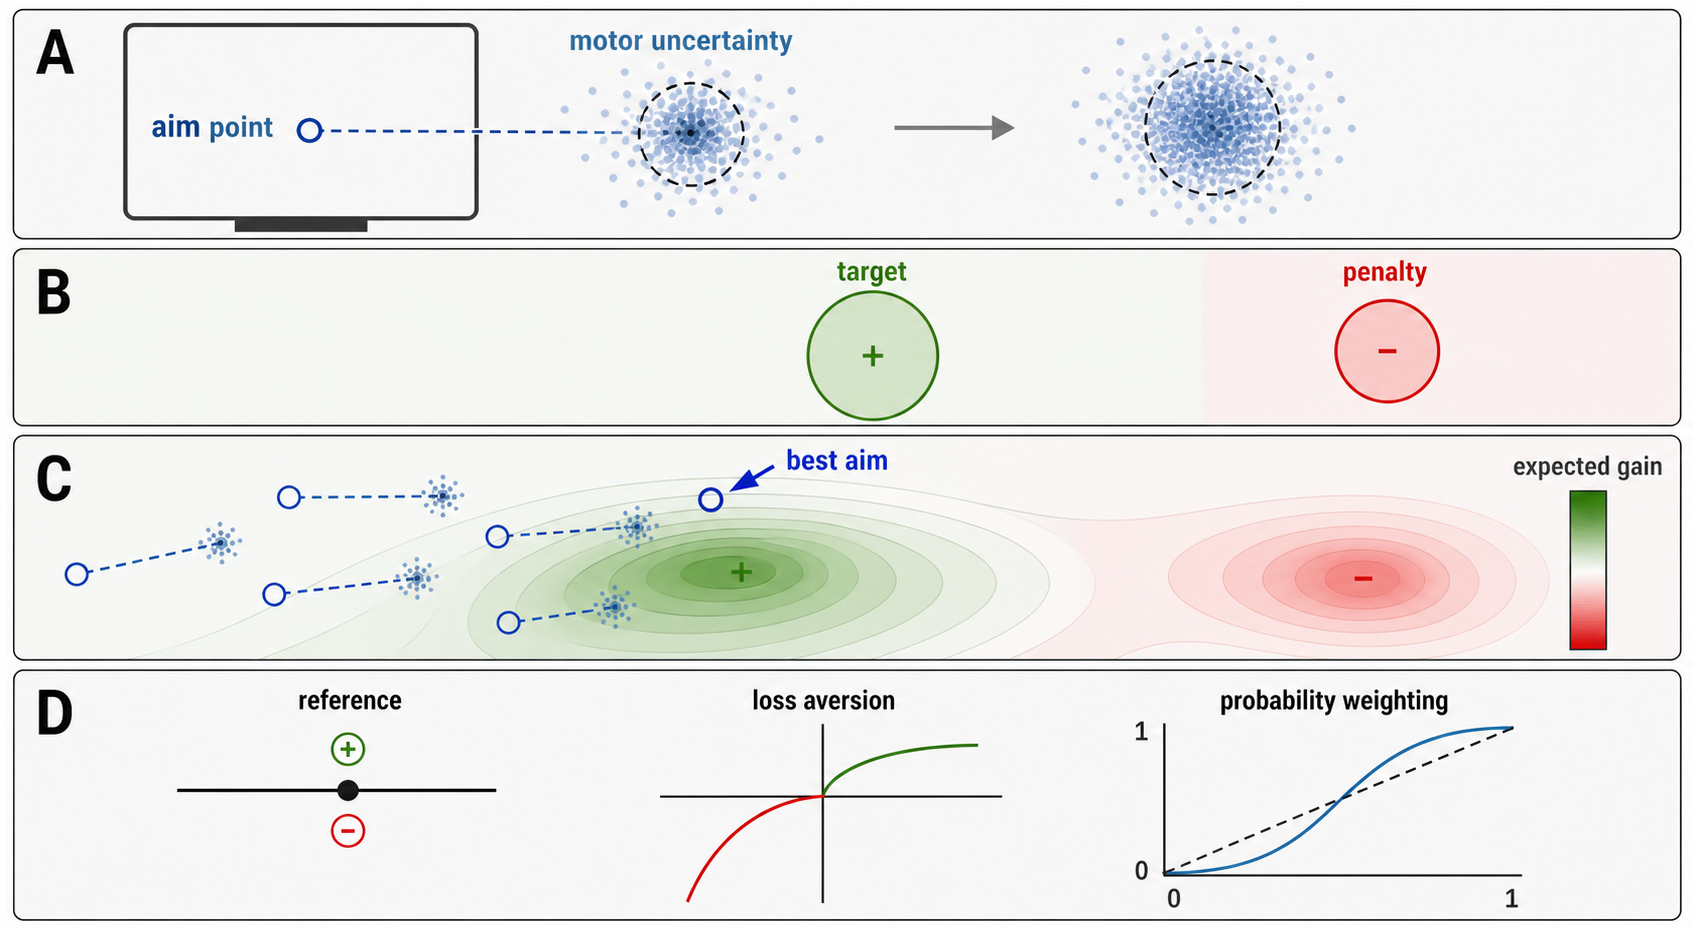
\includegraphics[width=0.96\textwidth]{figures/mhbf-lecture4-motor-lottery.png}
\caption{Continuous motor actions under uncertainty. An intended aim point generates a distribution of endpoints, reward and penalty regions assign gains and losses to those endpoints, the expected-gain landscape determines the best aim, and behavioral caveats such as reference dependence, loss aversion, and probability weighting can distort objective reward maximization.}
\end{figure}

The Trommershauser-style motor task in the Summer slides makes this concrete. Subjects touch a screen within a short deadline, such as 700 ms, and try to earn as much as possible. A hit in a green target region can produce a small gain, such as 2.5 cents, while a hit in a nearby red penalty region can produce a larger loss, such as 12.5 cents. Because endpoint variability is unavoidable, an aim point defines a lottery over possible regions:
\[
  L(a)
  =
  \bigl[P_a(R_1),G_1;\;P_a(R_2),G_2;\;\cdots;\;P_a(R_m),G_m\bigr].
\]
The probabilities \(P_a(R_i)\) are not subjective labels; they are the probabilities that the motor endpoint lands in region \(R_i\) when the chosen aim point is \(a\). The gains \(G_i\) are the objective payoffs attached to those regions. The expected gain is
\[
  Q(a)
  =
  \sum_{i=1}^{m}P_a(R_i)G_i.
\]
The best aim point need not be the center of the target. If the penalty region is close and costly, the expected-gain maximum shifts away from it. This is the movement version of a decision criterion shift: the policy changes because the payoff geometry changes.

The lecture also flags why human behavior may deviate from objective expected value. Prospect-theory-like effects can be summarized by replacing objective gains and probabilities with subjective ones:
\[
  U(a)
  =
  \sum_i \omega(P_a(R_i))\,v(G_i-r_0).
\]
The reference level \(r_0\) defines what counts as a gain or loss. The value function \(v\) can make losses larger in subjective magnitude than equal-sized gains, which is loss aversion. The weighting function \(\omega\) can overweight small probabilities or underweight large probabilities. These effects are suboptimal relative to objective expected reward, but they are systematic and therefore modelable.

\paragraph{Practical implication.}
For continuous decisions, do not ask only which target the subject wanted. Estimate the endpoint distribution, compute the expected-gain landscape, and compare the observed aim point with the expected-gain optimum. The residual tells you whether the subject's policy is near optimal, uses the wrong motor uncertainty, or values gains and losses nonlinearly.

\subsection{Signal detection theory: sensitivity versus criterion}

The problem solved by signal detection theory is to separate evidence quality from response criterion. The Summer deck lists several factors that influence decisions: signal strength relative to noise, sensitivity, signal frequency, motivation, costs for hits and false alarms, and personal bias. Signal detection theory gives a way to measure sensitivity even when the criterion moves.

Let \(s\in\{A,B\}\) again denote two states, such as signal present and signal absent. Let \(x\) be a scalar evidence variable. A criterion policy chooses \(A\) when \(x>c\) and \(B\) when \(x\le c\):
\[
  a(x)
  =
  \begin{cases}
    A, & x>c,\\
    B, & x\le c.
  \end{cases}
\]
The criterion \(c\) is a policy parameter. Moving it changes the mix of hits, misses, false alarms, and correct rejections without changing the sensory distributions.

\begin{figure}[!htbp]
\centering
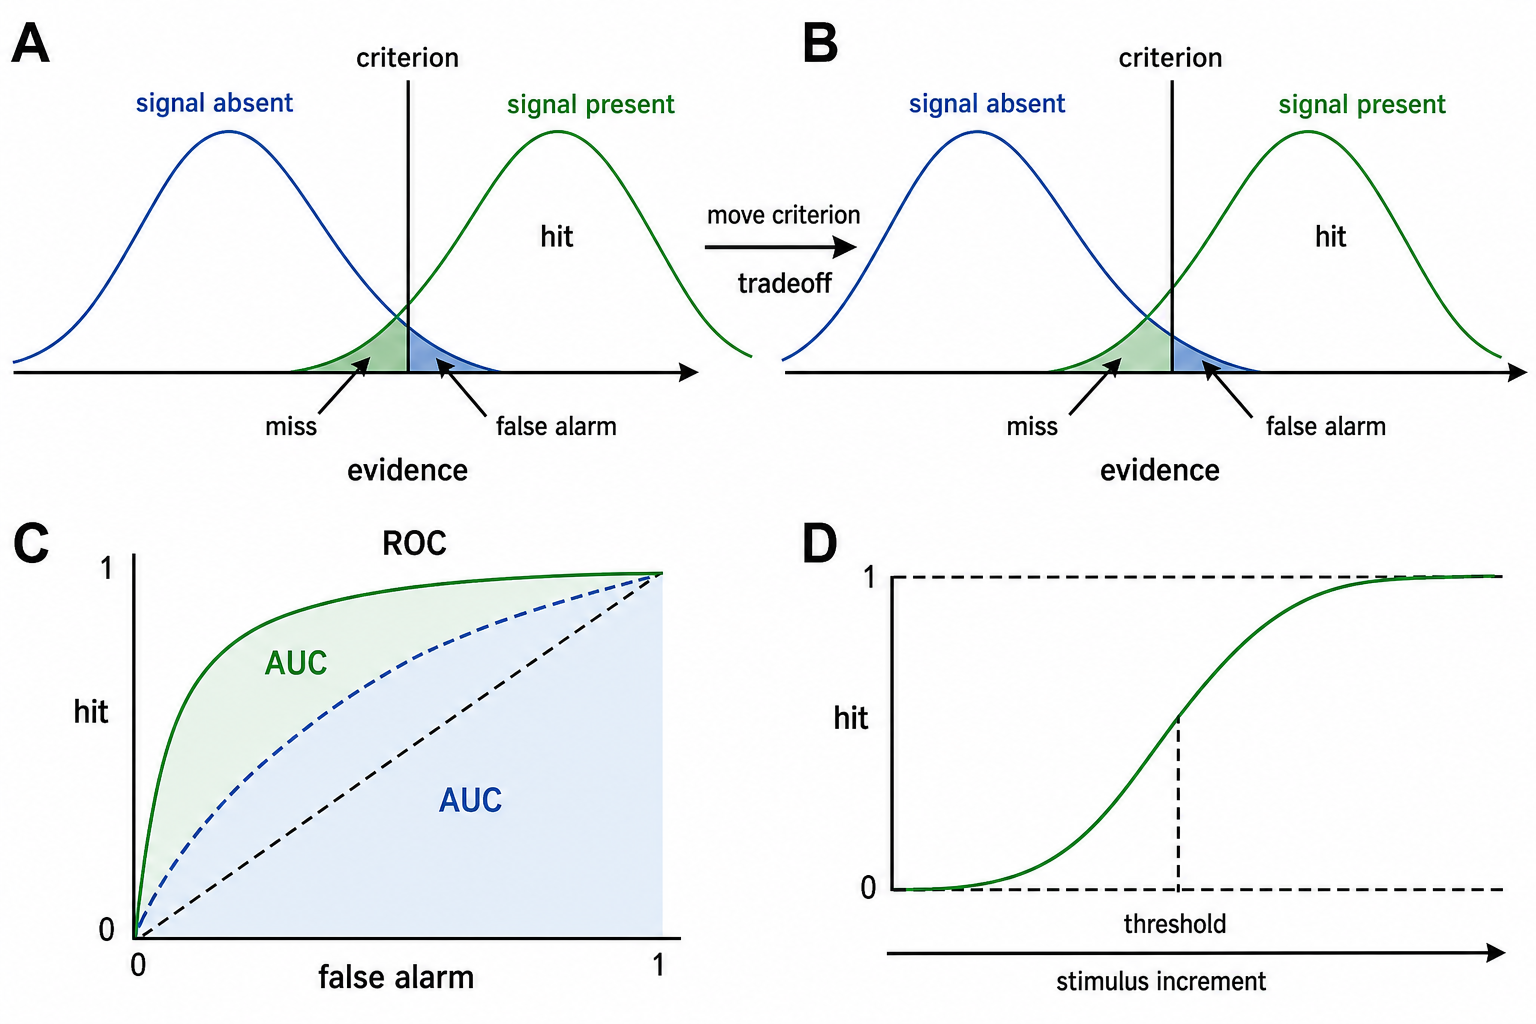
\includegraphics[width=0.96\textwidth]{figures/mhbf-lecture4-signal-detection.png}
\caption{Signal detection theory separates discriminability from criterion placement. Overlapping evidence distributions make errors unavoidable, the criterion controls the miss--false-alarm tradeoff, the ROC curve summarizes that tradeoff across criteria, and threshold functions are gradual because evidence varies across trials.}
\end{figure}

Under the standard equal-variance Gaussian model,
\[
  x\mid s=A \sim \mathcal N(\mu_A,\sigma^2),
  \qquad
  x\mid s=B \sim \mathcal N(\mu_B,\sigma^2),
  \qquad
  \mu_A>\mu_B,
\]
the sensitivity index is
\[
  d'
  =
  \frac{\mu_A-\mu_B}{\sigma}.
\]
It measures separation of the two evidence distributions in units of evidence noise. A large \(d'\) means the same criterion can achieve many hits with few false alarms. A small \(d'\) means errors are forced by overlap.

For a fixed criterion, define
\[
  H=P(x>c\mid s=A),
  \qquad
  F=P(x>c\mid s=B).
\]
\(H\) is the hit rate and \(F\) is the false-alarm rate. With unit-variance Gaussian evidence,
\[
  d'=\Phi^{-1}(H)-\Phi^{-1}(F).
\]
The inverse Gaussian CDF converts observed response probabilities back into evidence-axis coordinates. Their difference estimates the separation of the signal and noise distributions independently of the observer's particular criterion.

An ROC curve sweeps the criterion and plots hit rate against false-alarm rate. A curve near the diagonal indicates weak evidence. A curve bowed toward the upper-left corner indicates strong evidence. This is why the ROC is useful: it evaluates evidence quality without assuming that one observed criterion is the right one.

\paragraph{Practical implication.}
Hit rate alone is not a sensitivity measure. A liberal observer can have a high hit rate and a high false-alarm rate; a conservative observer can have a low hit rate and a low false-alarm rate. Sensitivity requires comparing both rates, or fitting the full response distribution.

\subsection{Sequential evidence accumulation}

The problem solved by sequential accumulation is that one sample of evidence is often not enough. The lecture's coin-flip example asks whether heads are more likely than tails. One unusually long run may be sufficient, but on many trials the observer should collect more samples before committing.

Let the hidden state \(s\) determine the probability of heads. For example,
\[
  s=A:\;p(\mathrm{heads})=0.3,
  \qquad
  s=B:\;p(\mathrm{heads})=0.7.
\]
At time \(n\), the evidence is the sequence \(x_{1:n}=\{x_1,\ldots,x_n\}\). The available actions are answer \(Y\), answer \(N\), or collect sample \(n+1\). The Summer deck assigns reward \(0\) for a correct answer, \(-1\) for a wrong answer, and \(-\kappa\) for another sample, with \(0<\kappa<1/2\). The sampling cost \(\kappa\) is the pressure toward stopping.

For conditionally independent evidence,
\[
  p(x_{1:n}\mid s)
  =
  \prod_{i=1}^{n}p(x_i\mid s).
\]
The posterior can be updated recursively:
\[
  p(s\mid x_{1:n})
  =
  \frac{p(x_n\mid s)p(s\mid x_{1:n-1})}{p^*(x_n)},
\]
where \(p^*(x_n)\) is the predictive probability of the new sample under the current belief. The important point is that the old posterior becomes the new prior.

\begin{figure}[!htbp]
\centering
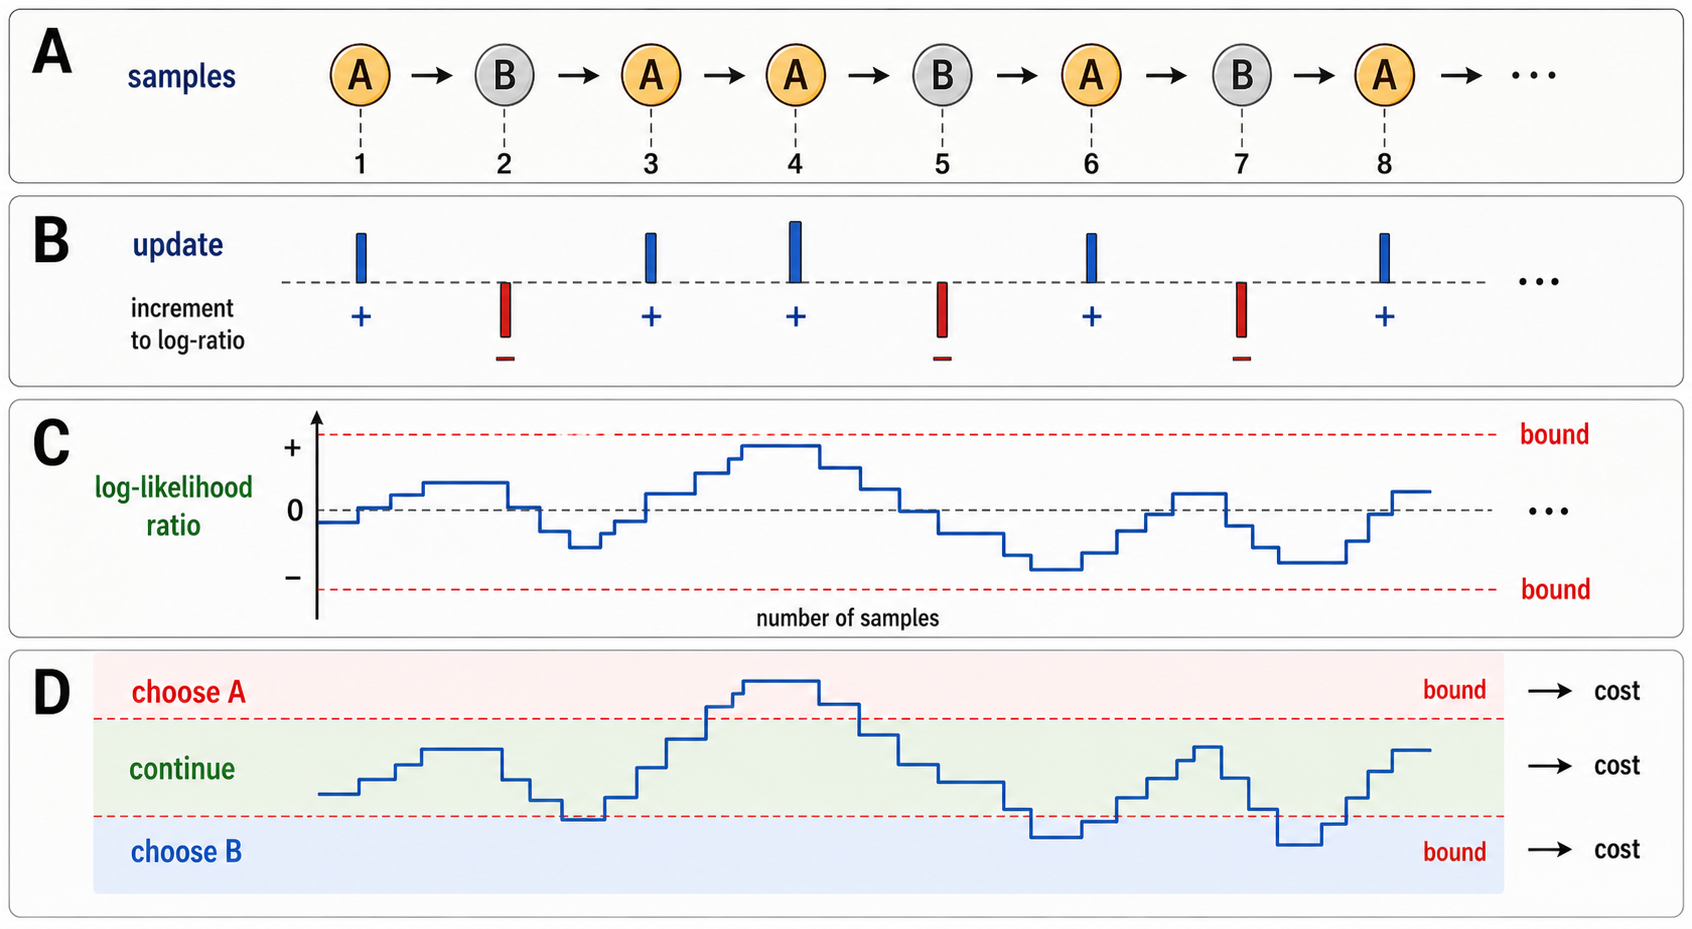
\includegraphics[width=0.96\textwidth]{figures/mhbf-lecture4-sequential-llr.png}
\caption{Sequential log-likelihood accumulation. Each sample contributes an additive update to the log-likelihood ratio, so posterior evidence evolves as a random walk. The policy has three regions: choose one state above the upper bound, choose the other below the lower bound, and continue sampling while the expected value of another sample exceeds its cost.}
\end{figure}

The clean state variable is the log-likelihood ratio
\[
  X_n
  =
  \log
  \frac{p(s=A\mid x_{1:n})}{p(s=B\mid x_{1:n})}.
\]
Using the recursive posterior update,
\[
  X_n
  =
  \log
  \frac{p(x_n\mid s=A)}{p(x_n\mid s=B)}
  +
  X_{n-1}.
\]
This is the mechanism behind accumulation. The retained state variable \(X_n\) does not need to store every previous sample. It stores the accumulated log evidence, and each new sample adds one log-likelihood increment.

For Gaussian likelihoods with unit variance and means \(\pm d'/2\),
\[
  p(x\mid s=A/B)
  =
  \frac{1}{\sqrt{2\pi}}
  \exp\!\left[-\frac{(x\mp d'/2)^2}{2}\right],
\]
the increment is
\[
  \log\frac{p(x_n\mid s=A)}{p(x_n\mid s=B)}
  =
  d'x_n,
\]
so
\[
  X_n=X_{n-1}+d'x_n.
\]
Positive samples move the belief toward \(A\), negative samples move it toward \(B\), and noisy samples make \(X_n\) a random walk with drift.

\subsection{Stopping rules and decision bounds}

The problem solved by a stopping rule is deciding when uncertainty is low enough. If \(|X_n|\) is large, one posterior dominates and the probability of choosing incorrectly is small. If \(|X_n|\) is near zero, the two states remain similarly plausible and more evidence may be worth the cost.

If the observer chooses the state with the larger posterior, the probability of being wrong is
\[
  P(\mathrm{wrong}\mid X_n)
  =
  \frac{1}{1+e^{|X_n|}}.
\]
Because a wrong answer pays \(-1\), the expected reward of stopping and choosing the more likely state is
\[
  \langle R\rangle_{\mathrm{stop}}
  =
  -\frac{1}{1+e^{|X_n|}}.
\]
The immediate reward of collecting one more sample is \(-\kappa\), ignoring future benefits beyond the next sample. Stopping becomes better than continuing when
\[
  -\frac{1}{1+e^{|X_n|}}
  >
  -\kappa.
\]
Equivalently,
\[
  |X_n|
  >
  a_\kappa,
  \qquad
  a_\kappa
  =
  \log\frac{1-\kappa}{\kappa}.
\]
The two decision bounds are therefore \(\pm a_\kappa\). A smaller sampling cost raises the bound, because it is cheap to wait. A larger sampling cost lowers the bound, because the observer should commit with less evidence.

\paragraph{Practical implication.}
Sequential decision data contain more information than final choice alone. Accuracy estimates the sign and scale of drift, reaction times estimate bound height and noise, and changes in deadline or sampling cost should move the bound even when sensory evidence is unchanged.

\subsection{Drift-diffusion as the continuous limit}

The problem solved by the drift-diffusion model is to connect discrete Bayesian updating with the smooth reaction-time distributions measured in psychophysical tasks. When many small evidence samples arrive rapidly, the log-likelihood random walk can be approximated by a stochastic differential equation:
\[
  dX_t
  =
  \mu\,dt
  +
  \sigma\,dW_t,
  \qquad
  X_0=z.
\]
\(X_t\) is the retained decision variable. The drift \(\mu\) is the average evidence rate, the diffusion scale \(\sigma\) is within-trial evidence noise, and \(z\) is the starting point or initial bias. A decision is made when
\[
  X_t=+a
  \qquad\text{or}\qquad
  X_t=-a.
\]
The bound height \(a\) controls the speed-accuracy tradeoff. Higher bounds require more evidence and tend to increase accuracy and reaction time. Lower bounds produce faster but less reliable decisions.

The random-dot motion slide in the Summer deck is a behavioral assay for this idea. Motion strength is the percentage of coherently moving dots. Higher coherence increases the evidence rate, so percent correct rises and mean reaction time falls. In model terms, coherence changes \(\mu\), while instructions about speed or caution change \(a\).

\begin{figure}[!htbp]
\centering
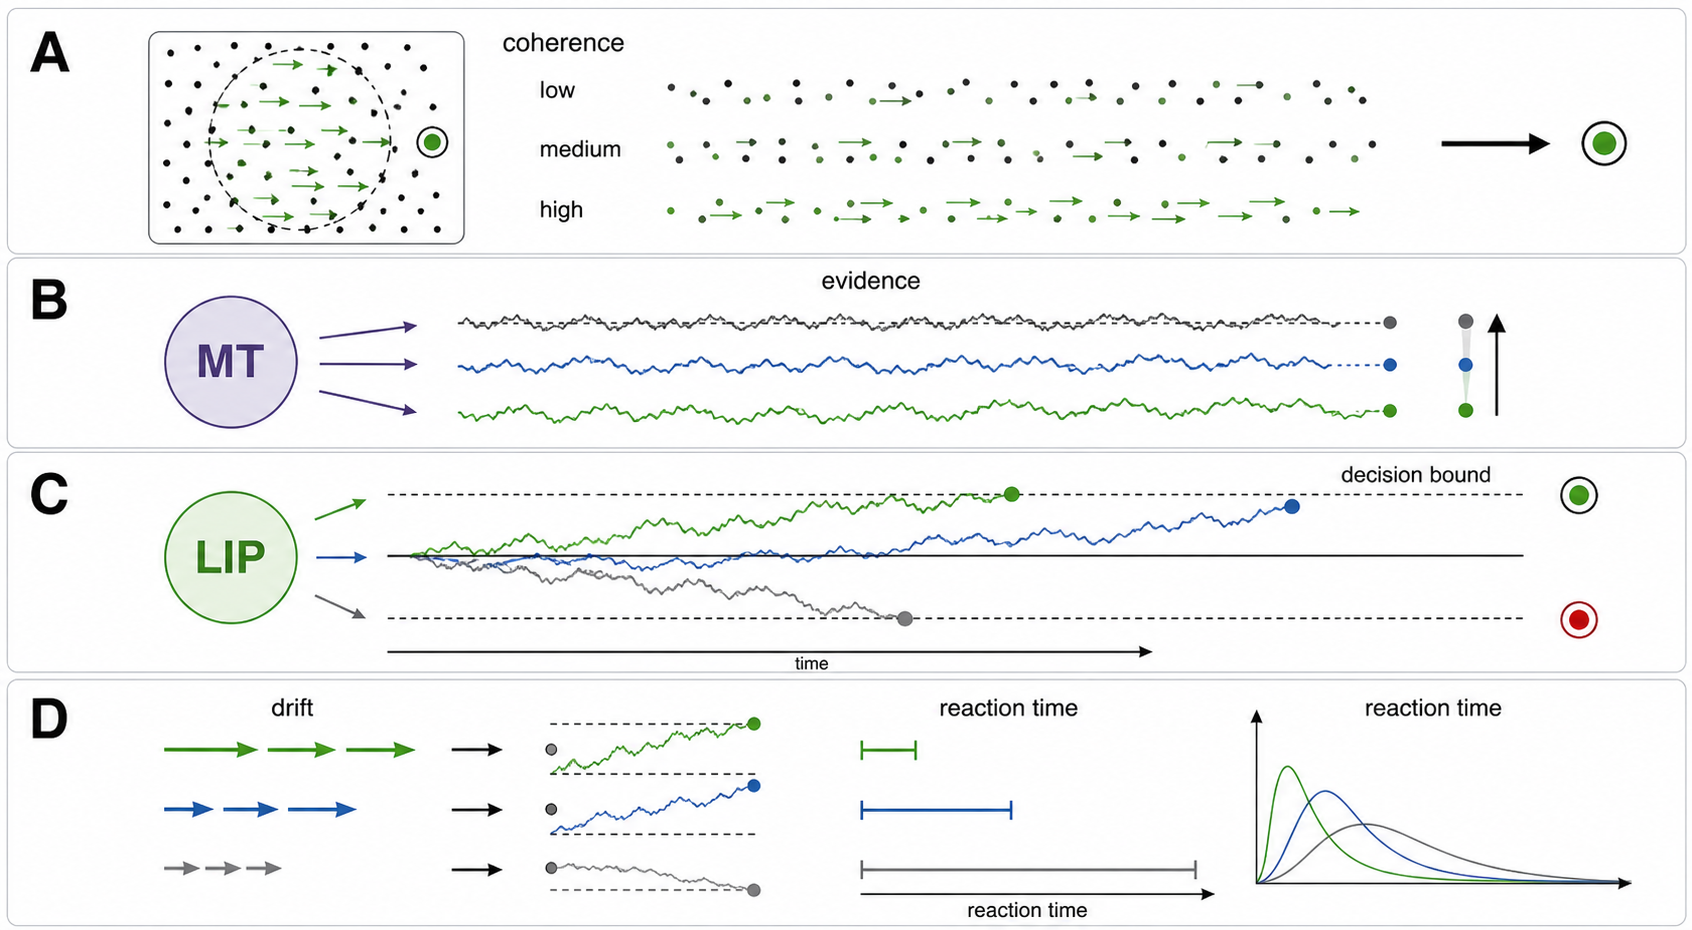
\includegraphics[width=0.96\textwidth]{figures/mhbf-lecture4-evidence-accumulation.png}
\caption{Evidence accumulation in random-dot decisions and the neural extension. Motion coherence controls the strength of momentary evidence, noisy evidence is integrated into a decision variable, a decision is made when the variable reaches a bound, and variability in drift or noise produces broad reaction-time distributions. In the archival neurophysiology framing, MT supplies motion evidence and LIP represents target-linked accumulated evidence.}
\end{figure}

The Summer deck also notes that extended DDMs often include variability in starting point and mean drift. This is not a cosmetic addition. Starting-point variability can explain response bias and fast errors, while drift variability can broaden the reaction-time distribution and produce asymmetries between correct and error trials.

\paragraph{Archival neural extension.}
The earlier archive material and the standard Gold-Shadlen framing connect the same computational variables to neural measurements. MT responses can be treated as momentary motion evidence, while LIP activity can be treated as a target-linked accumulated decision variable. Neurometric thresholds ask whether neural responses contain enough information to support behavior, and microstimulation manipulations ask whether changing sensory evidence or decision state causally shifts choices. This material is useful for course integration, but it should be read as a neural extension rather than as the core content of the Summer Lecture 4 deck.

\paragraph{Practical implication.}
For a decision-making experiment, fit both choices and reaction times. A model that predicts percent correct but ignores the time to bound crossing has left out the main observable that distinguishes drift changes from bound changes.

\subsection{Ballistic accumulation and heavy-tailed reaction times}

The analytical tutorial introduces a simpler model that isolates one mechanism for broad reaction-time distributions. In a linear ballistic accumulator, the decision variable is noiseless within a trial:
\[
  dX=\mu\,dt,
  \qquad
  X(0)=0.
\]
The drift \(\mu\) is drawn independently on each trial,
\[
  \mu\sim \mathcal N(\mu_0,\sigma_\mu^2).
\]
The bounds are at \(\pm a\). If \(\mu_0>0\), the upper bound is the correct bound. The probability of a correct decision is
\[
  P(\mathrm{correct})
  =
  P(\mu>0)
  =
  \Phi\!\left(\frac{\mu_0}{\sigma_\mu}\right).
\]
Accuracy therefore depends on the mean drift in units of trial-to-trial drift variability.

For a given positive drift, the reaction time to the upper bound is
\[
  T(\mu)=\frac{a}{\mu}.
\]
Fast drifts give short reaction times, and small positive drifts give very long reaction times. The variable transformation \(\mu=a/T\) first gives the unnormalized correct-response mass
\[
  p_T^{+}(T)
  =
  p_\mu(a/T)\frac{a}{T^2},
  \qquad
  T>0.
\]
The superscript \(+\) means that this is the joint density of reaction time and an upper-bound crossing. It integrates to \(P(\mu>0)\), not to one. The normalized reaction-time density conditional on a correct response is therefore
\[
  p(T\mid \mathrm{correct})
  =
  \frac{p_\mu(a/T)}{P(\mu>0)}\frac{a}{T^2},
  \qquad
  T>0.
\]
If one pools both upper- and lower-bound crossings, the corresponding normalized density is branched by the sign of \(\mu\):
\[
  p_{\mathrm{all}}(T)
  =
  \frac{a}{T^2}
  \left[
    p_\mu(a/T)+p_\mu(-a/T)
  \right],
  \qquad
  T>0.
\]
As \(T\to\infty\), the argument \(a/T\to 0\). For correct trials,
\[
  p(T\mid \mathrm{correct})
  \approx
  \frac{a\,p_\mu(0)}{P(\mu>0)\,T^2}.
\]
For all crossings, the tail has the same exponent, \(p_{\mathrm{all}}(T)\approx 2a\,p_\mu(0)/T^2\), when \(p_\mu\) is continuous at zero. The \(T^{-2}\) tail makes the mean reaction time diverge logarithmically in the idealized model. Real experiments have deadlines, lapses, and physiological constraints, so the literal infinity is not the point. The point is that drift variability can make sample means unstable unless the full reaction-time distribution is modeled.

\subsection{How Decision Making I fits the course}

Decision making turns the course's latent-state theme into an action rule:
\[
  \text{hidden state}
  \rightarrow
  \text{noisy evidence}
  \rightarrow
  \text{posterior or decision variable}
  \rightarrow
  \text{policy}
  \rightarrow
  \text{action}.
\]
The same structure appeared in multisensory integration as reliability-weighted inference. Here the additional ingredient is reward. The posterior says what is probable; the policy says what is worth doing.

\begin{center}
\begin{tabular}{lp{0.62\textwidth}}
\hline
Concept & Role in the lecture \\
\hline
Prior \(p(s)\) & belief about hidden states before the current evidence \\
Likelihood \(p(x\mid s)\) & measurement model for evidence under each state \\
Posterior \(p(s\mid x)\) & belief state after observing evidence \\
Reward \(R(s,a)\) & payoff for action \(a\) in state \(s\) \\
Policy \(\pi(a\mid x)\) & rule mapping evidence or belief to action \\
Motor lottery \(L(a)\) & endpoint probabilities and gains induced by an intended movement \\
Criterion \(c\) & evidence value where two actions have equal expected reward \\
\(d'\) & separation of evidence distributions in noise units \\
ROC curve & criterion-sweep summary of evidence quality \\
Log-likelihood ratio \(X_n\) & retained sequential evidence for one state over another \\
Decision bound \(a\) & stopping threshold controlling the speed-accuracy tradeoff \\
Drift \(\mu\) & mean evidence accumulation rate \\
\hline
\end{tabular}
\end{center}

\subsection{Conceptual takeaways from Lecture 4}

\begin{itemize}
    \item Bayesian decision making chooses actions by expected reward, not by posterior probability alone.
    \item Priors, likelihoods, rewards, and policies have different roles and should not be collapsed into one vague notion of bias.
    \item Continuous movements are decisions because an aim point creates a probability distribution over rewarded and penalized outcomes.
    \item Motor lotteries explain why the optimal aim can shift away from the target center when motor uncertainty and penalties are asymmetric.
    \item Prospect-theory caveats are systematic deviations from objective expected reward, not random noise.
    \item Signal detection theory separates sensitivity from criterion by comparing hits and false alarms.
    \item ROC curves summarize evidence quality across criteria.
    \item Sequential Bayesian updating is additive in the log-likelihood ratio.
    \item Sampling costs turn posterior uncertainty into decision bounds.
    \item Drift-diffusion models use the retained decision variable to explain both accuracy and reaction-time distributions.
\end{itemize}

\subsection*{Sources used for Lecture 4}

\begin{itemize}
    \item J.-D. Haynes, Summer 2026 ``Lecture 4 - Decision making I'' slide deck, 30 pages, extracted locally from the course slide PDF.
    \item Models of Higher Brain Function Analytical Tutorial, Exercise 4: Decision Making I, May 22, 2026, extracted locally from the analytical tutorial PDF.
    \item Course archive decision-making material, used only for the explicitly marked archival neural extension connecting random-dot decisions to MT/LIP, neurometric thresholds, and microstimulation.
    \item Trommersh\"auser et al. (2008), motor uncertainty and reward-function examples as reproduced in the Summer deck.
    \item Gold and Shadlen (2007), drift-diffusion and random-dot decision framing as cited in the Summer deck.
\end{itemize}
